\section{Abstract Syntax Tree}
\label{sec:AST}
As described in section \ref{sec:compiler}, the parser generates an \textit{abstract syntax tree} (AST). An AST is a representation of the syntax in a programming language in the structure of a tree. Each node of the tree represents a token in the given sentence or code block. Since the tree is abstract not every single syntactic construct is shown in the tree. As javaCC is used in the creation of this project, the AST is generated automatically based on the grammar of BAL.

\subsection{AST for Function and Variable Declaration}
\begin{lstlisting}[caption=Different variable declarations and a function call, label=lst:ast_func]
	float f = 1.421 + 3;
	string hello = "World";
	call system.out.print("parameter");
\end{lstlisting}
\begin{figure}[H]
	\centering
		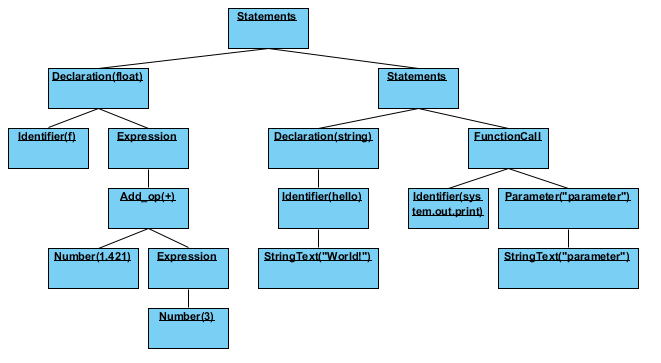
\includegraphics[width=\textwidth]{billeder/function_AST.png}
		\caption{AST for listing \ref{lst:ast_func}}
		\label{fig:ast_func}
\end{figure}
In listing \ref{lst:ast_func} is seen two different variable declarations in BAL, a float, which consist of the arithmetic operation addition, and a string, which contains the word ''world``. In the same listing a function call is shown, which has a string parameter called "parameter". Figure \ref{fig:ast_func} shows the AST generated by javaCC using the before mentioned code example. It is not concrete to the specific token. As seen in the AST there are different opportunities for declaring a variable in BAL. For example, an expression can be either an arithmetic operator, which contains a new expression, or a number to define the variable.

\subsection{AST for While Loops and If Statements}
\begin{lstlisting}[caption=While loop with if-statement, label=lst:ast_while]
	while(b <= 1) do
		if(a EQUALS s) do
			string hello = "World!";
		end
	end
\end{lstlisting}
\begin{figure}[H]
	\centering
		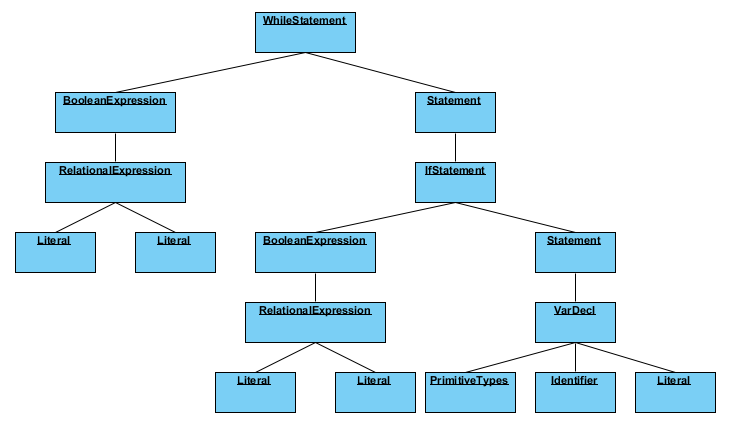
\includegraphics[width=\textwidth]{billeder/while_AST.png}
		\caption{AST for listing \ref{lst:ast_while}}
		\label{fig:ast_while}
\end{figure}
In listing \ref{lst:ast_while} is seen a while loop with an if-statement, containing a variable declaration, in BAL. Figure \ref{fig:ast_while} shows the AST generated from the code example. As seen in the AST, the while loop and the if-statement have different boolean expressions to. The while loop checks if an identifier is less than or equal to a number, and the if-statement checks if two identifiers are equal.